\documentclass[../main.tex]{subfiles}

\begin{document}
    \begin{center}
        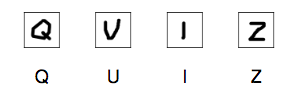
\includegraphics[width=0.5\textwidth,height=0.5\textheight,keepaspectratio]{scribe_qviz}
    \end{center}

    We can form a scoring function $F(w, x, y_1, \dots, y_4)$ by defining scoring functions over not just each $y_i$ for $i \in \{1,2,3,4\}$ but over pairs of the $y_i$. For example, we define a scoring function over $(y_1,y_2)$, $(y_2,y_3)$ and $(y_3,y_4)$. Formally, we obtain;

    \begin{equation}
        F(w, x, y_1, \dots, y_4) = f_1(w,x,y_1) + f_2(w,x,y_2) + f_3(w,x,y_3) + f_3(w,x,y_4) + \\ f_{1,2}(w,x,y_1,y_2) + f_{2,3}(w,x,y_2,y_3) + f_{3,4}(w,x,y_3,y_4) \tag{$\alpha$}
    \end{equation}

    This captures our intuition that there is structure in the choice of consecutive letters in a word. For example, a word in english beginning with $Q$ is far more likely to be followed by $U$ than by $V$. \\

    Optimizing over this new scoring function also decreases the size of the argument space \footnote{Argument space was not a term used in lecture; we use it to refer to the space of values that our scoring algorithm maximizes over}. Formerly, when we were maximizing \\

    \[
        F(w, x, y_1 \dots y_4) = \sum_{D \in \text{(Letter Set)}^4}^{} f_d(w,x,y_1,y_2,y_3,y_4)
    \]

    where Letter Set refers to the 26 letters in English, we were maximizing over an argument space $26^4$ in size. The argument space of $(\alpha)$, by contrast, is 

    \[
        26^2(3) + 26(4) \qquad \text{-- There are 3 pairs of 2 letters and 4 single letters}
    \]

    We can visualize our new scoring function as a graph. Notice that, for this problem,
    the graph is a tree. This will become important later.

    \begin{center}
        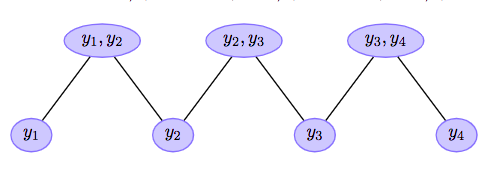
\includegraphics[width=0.5\textwidth,height=0.5\textheight,keepaspectratio]{scribe_qviz_graph}
    \end{center}

    In summary, our scoring function can employ special cases by:

    \begin{outline}
        \1 Defining the scoring function as a sum of composite scoring functions, where
        each composite function's argument space solely considers one variable.
        \2 
        \[
            F(w, x, y_1 \dots y_d) = \sum_{i=1}^{d}f_i(w,x,y_d)
        \]
        \1 Defining the scoring function as a sum over all possible members of the
        argument space.
        \[
            F(w, x, y_1 \dots y_d) = f_{1 \dots D}(w,x,y_1, \dots, D)
        \]
    \end{outline}

    More generally, we can define a scoring function as a sum of composite scoring
    functions, and each composite considers \textit{some} subset of the entire argument space.
    \begin{example}

    A task in computer vision is to delineate the boundaries of distinct figures in a picture. For example, we would like to be able to segregate the bikers and bikes appearing in the picture below.

    \begin{center}
        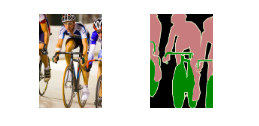
\includegraphics[width=0.5\textwidth,height=0.5\textheight,keepaspectratio]{semantic_sep_example}
    \end{center}

    Supposing that there are $D$ class labels that we wish to assign to any given pixel $x$ in the image above, then we can do this by defining a scoring function over the labels like

    \[
        \sum_{i=1}^{D}f_d(w, x, y_d) + \sum_{i,j}^{}f_{i,j}(w,x,y_i,y_j)
    \]

    The functions whose argument space is the range of one label (a unary term) are referred to as image evidence terms and the functions with pairwise terms are called smoothness priors. In most natural images, neighboring pixels resemble each other, so the smoothness priors give a higher score to labels that resemble each other. This disposition -- to give similar, neighboring pixels a higher score -- makes the prediction labels appear smooth, which is why these terms are called smoothness priors.

    In contrast to the graph presented for the QVIZ example, it is also a pattern to represent a scoring function by letting unary terms be vertices and letting composite terms be edges between vertices.

    \begin{center}
        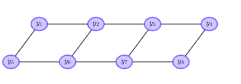
\includegraphics[width=0.5\textwidth,height=0.5\textheight,keepaspectratio]{semantic_sep_graph}
    \end{center}
        
    \end{example}

    \subsection{Techniques for Identifying the Higest Scoring Configuration:}

    There are a few candidates for inference algorithms:

    \begin{outline}
    \1 Exhaustive Search \\
    \1 Dynamic Programming \\
    \1 Integer Linear Program \\
    \1 Linear Programming Relaxation \\
    \1 Message Passing \\
    \1 Graph Cut \\
    \end{outline}

    We will touch upon exhaustive search, dynamic programming and message passing.

\end{document}
